\documentclass[a4paper,11pt,fleqn]{article}%fleqn pour aligner les equations à gauche
\usepackage{../../Styles/Exercice}


\newcommand{\chnum}{Chapitre 3}
\newcommand{\chtitle}{Cinétique chimique}
\newcommand{\dtype}{Exercices}
  

\begin{document}
\maketitle
\begin{multicols}{2}
\section{Identifier un facteur cinétique}
Les mélanges ci-dessous sont réalisés à partir d'une solution de concentration en quantité d'iodure de potassium $C_1$ = \num{0,20} \unit{\mole\per\liter} et d'une solution de concentration en quantité d'acide sulfurique $c_2$ = \num{0,50} \unit{\mole\per\liter}.
\begin{center}
    \begin{tabular}{|>{\centering}m{.2\linewidth}|>{\centering}m{.2\linewidth}|>{\centering}m{.2\linewidth}|>{\centering\arraybackslash}m{.2\linewidth}|}
    \hline Mélange & n°1 & n°2 & n°3\\
    \hline $V_1$ (en \unit{\milli\liter}) & 10 & 20 & 30\\
    \hline $V_2$ (en \unit{\milli\liter}) & 10 & 10 & 10\\
    \hline $V_3$ (en \unit{\milli\liter}) & 30 & 20 & 10\\
    \hline
    \end{tabular}
\end{center}

$V_1$ désigne le volume de solution d'iodure de potassium, $V_2$ le volume de solution d'acide sulfurique et $V_3$ le volume d'eau ajoutée.\\
Au même instant, dans chaque bécher est versé une solution de concentration en quantité de péroxyde d'hydrogène $c_4$ = \num{10} \unit{\milli\mole\per\liter} et de volume $V_4$ = \num{50} \unit{\milli\liter}. Au bout de deux minutes, la coloration jaune (caractéristique de la présence de diiode) est de plus en plus foncée du bécher 1 au bécher 3.\\
L'équation de la réaction qui modélise la transformation est :
$$\small \ce{H2O2(aq) + 2H+(aq) + 2I-(aq) -> 2H2O(l) + I2(aq)} $$
\begin{enumerate}
    \item Expliquer les colorations de plus en plus foncées observées au même instant du bécher 1 au bécher 3.
    %\textcolor{blue}{Les colorations foncées viennent de l'apparition de diiode dans chaque bécher à des vitesses différentes.}
    \item Montrer que, quel que soit le mélange, le réactif limitant est le peroxyde d'hydrogène \ce{H2O2}.
    %\textcolor{blue}{On constate que, quelle que soit le mélange les quantités d' peroxyde d'hydrogène est la même : $n_{\ce{H2O2}} = c_4 \times V_4 = \num{10e-3} \times \num{50e-3}$ = \num{5,0e-4} \unit{\mole}. %\textcolor{olive}{$x_{max}$ = \num{5,0e-4} \unit{\mole}}\\
    %de même la quantité d'acide sulfurique est la même dans chaque expérience :\\
    %$n_{\ce{H+}} = c_2 \times v_2 = \num{0,50} \times \num{10e-3}$ = \num{5,0e-3} \unit{\mole}. \textcolor{orange}{$x_{max}$ = \num{2,5e-3} \unit{\mole}}\\
    %Il ne reste que la quantité d'ions iodure à déterminer : }
    %\begin{tabular}{|c|c|c|}
    %\hline Mélange & $n_{\ce{I-}}$ & $x_{max}$\\
    %\hline 1 & \num{2e-3} & \num{1e-3}\\
    %\hline 2 & \num{4e-3} & \num{2e-3}\\
    %\hline 3 & \num{6e-3} & \num{3e-3}\\
    %\hline
   % \end{tabular}\\
    %\textcolor{blue}{On constate que la valeur de $x_{max}$ la plus faible est toujours celle du peroxyde d'hydrogène, il sera donc le réactif limitant dans chacun des cas.}
    \item En déduire la quantité de matière, puis la concentration en quantité de diiode finales dans chaque mélange.
    \item Déterminer alors s'il subsiste une différence d'intensité de coloration d'un bécher à un autre.
\end{enumerate}

\section{Stabilité de l'eau de Javel}
L'eau de Javel (solution d'hypochlorite de sodium (\ce{Na+(aq)},\ce{Cl-(aq)}), solution désinfectante, doit être conservée au frais, à l'abri de l'air et de la lumière. En effet, l'ion hypochlorite se transforme selon la réaction d'équation :
\begin{eqnarray}
    \ce{2ClO-(aq) -> 2Cl-(aq) + O2(g)}\nonumber
\end{eqnarray}
La concentration en quantité d'ion hypochlorite d'un flacon d'eau de Javel est donnée ci-dessous à différentes dates pour deux solutions $S_1$ et $S_2$ différentes (à la température de \num{20} \unit{\celsius}).
\\
    \begin{tabular}{|c|c|c|c|c|c|c|}
    \hline t (en jours) & 0 & 50 & 100 & 150 & 200 \\
    \hline $c_1$ (en \unit{\mole\per\liter}) & 2,00 & 1,65 & 1,36 & 1,12 & 0,92\\
    \hline $c_2$ (en \unit{\mole\per\liter}) & 1,60 & 1,32 & 1,09 & 0,89 & 0,74\\
    \hline
    \end{tabular}\\
\noindent
    \begin{tabular}{|c|c|c|c|c|c|}
    \hline t (en jours) & 250 & 300 & 350 & 400\\
    \hline $c_1$ (en \unit{\mole\per\liter}) & 0,76 & 0,63 & 0,52 & 0,42\\
    \hline $c_2$ (en \unit{\mole\per\liter}) & 0,61 & 0,50 & 0,41 & 0,34\\
    \hline
    \end{tabular}
\begin{enumerate}
    \item Proposer une argumentation permettant de déterminer s'il est préférable de conserver des solutions d'eau de Javel concentrées ou diluées.
    \item Proposer une expérience permettant de vérifier la recommandation faite par le fabricant de conserver l'eau de Javel au frais.
    \item Dessiner l'allure des courbes attendues lors de cette expérience.
\end{enumerate}

\section{Transformer des gaz}
Le pentoxyde de diazote de formule \ce{N2O5} permet de réaliser des réactions chimiques de nitration pour l'obtention d'espèces explosives, comme le TNT. Le suivi temporel de sa décomposition à \num{343} \unit{\kelvin} est effectué dans une enceinte fermée de volume constant par mesure de la pression $P$ au cours du temps. Cette décomposition est modélisée par la réaction d'équation :
\begin{eqnarray}
    \ce{2N2O5(g) -> 4NO2(g) + O2(g)}\nonumber
\end{eqnarray}
Les résultats obtenus sont donnés ci-dessous.
\begin{center}
    \begin{tabular}{|c|c|c|c|c|c|}
    \hline $t$ (en min) & 0 & 10 & 20 & 30 & 40\\
    \hline $P$ (en bar) & 0,354 & 0,490 & 0,593 & 0,670 & 0,726\\
    \hline
    \end{tabular}
    \begin{tabular}{|c|c|c|c|c|c|}
    \hline $t$ (en min) & 50 & 60 & 70 & 80 & 100\\
    \hline $P$ (en bar) & 0,764 & 0,794 & 0,820 & 0,837 & 0,858\\
    \hline
    \end{tabular}
\end{center}

\textbf{Données :}\\
\begin{itemize}
    \item La concentration en quantité de matière d'une espèce gazeuse est définie par : $[\ce{N2O5}] = \dfrac{n_{\ce{N2O5}}}{V}$ où $V$ est le volume du gaz.
    \item Une analyse permet d'établir : $[\ce{N2O5}] = \dfrac{5P_0-2P}{3RT}$ avec $P_0$ la pression initiale en \unit{\pascal} (1 bar = \num{1e5} \unit{\pascal}), $R$ = \num{8,31} \unit{\joule\per\mole\per\kelvin}, $T$ la température  en kelvin et [\ce{N2O5}] en \unit{\mole\per\meter\cubed}.
\end{itemize}
\begin{enumerate}
    \item Calculer la vitesse volumique de consommation de \ce{N2O5} à $t$ = 0.
    \item Vérifier que l'évolution de [\ce{N2O5}] suit une loi de vitesse d'ordre 1.
\end{enumerate}

\section{Modéliser un nuage de points}
La décomposition de l'iodure d'hydrogène est modélisée par la réaction d'équation :
\begin{eqnarray}
    \ce{2HI(g) -> H2(g) + I2(g)}\nonumber
\end{eqnarray}
Le suivi temporel de cette transformation donne, à \num{580} \unit{\kelvin}, les résultats suivants :
\begin{center}
    \begin{tabular}{|>{\centering}m{.15\linewidth}|c|c|c|c|c|}
    \hline Temps (en s) & 0 & 1000 & 2000 & 3000 & 4000\\
    \hline [\ce{HI}] (en \unit{\mole\per\liter}) & 1,000 & 0,110 & 0,061 & 0,041 & 0,031\\
    \hline
    \end{tabular}
\end{center}
La concentration en quantité de matière d'une espèce gazeuse est définir comme celle d'une espèce dissoute : $[\ce{HI}] = \dfrac{n_{\ce{HI}}}{V}$ où $V$ est le volume du gaz et $[\ce{HI}]_0 = [\ce{HI}](0)$.
\begin{enumerate}
    \item Calculer, pour chaque date ci-dessus, $\ln{\dfrac{[\ce{HI}](t)}{[\ce{HI}]}}$.
    \item À l'aide d'une représentation graphique, déterminer si l'évolution de la concentration du iodure d'hydrogène suit une loi de vitesse d'ordre 1.
\end{enumerate}

\section{Purification de l'eau}
L'ozone \ce{O3} est utilisé dans le traitement de l'eau, pour la production d'eau potable et pour l'épuration des eaux industrielles. Lors du processus de purification, l'ozone est transformé en dioxygène, transformation modélisée par la réaction d'équation :
\begin{eqnarray}
    \ce{O3(aq) ->} \frac{3}{2} \ce{O2(aq)}\nonumber
\end{eqnarray}
L'évolution de la concentration en masse en ozone au cours du temps pour diverses concentrations en masse initiales en ozone dissous en présence de charbon actif est donnée ci-dessous (à la température de 20\unit{\celsius}).
\begin{center}
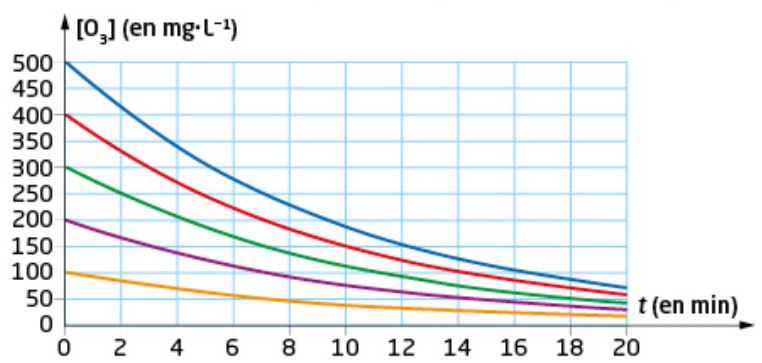
\includegraphics[width =\linewidth]{Ressources/TSPE_C10_Exercices_Fig1.png}
\end{center}
Par ailleurs, à la température de 20\unit{\celsius} en l'absence de charbon actif, le temps de demi-réaction vaut \num{13,1} \unit{\minute}.
\begin{enumerate}
    \item Déterminer, pour chaque concentration initiale, le temps de demi-réaction.
    \item En déduire si l'évolution de la concentration en quantité d'ozone suit ou ne suit pas une loi d'ordre 1.
    \item Indiquer quel est le rôle du charbon actif.
\end{enumerate}

\section{Un initiateur de polymère}
Le péroxyde de di\textit{tert}butyle, noté \textbf{A} est un amorceur de nombreuses réactions de polymérisation formant des matières plastiques.\\
Cette espèce chimique ne peut pas être utilisée à une température trop élevée car elle se décompose spontanément. Cette décomposition est modélisée par la réaction d'équation :
$$\tiny \ce{(H3C)3COOC(CH3)3(g) -> 2CH3COCH(g) + H3CCH3(g)}$$
La mesure de la pression totale $P$ du mélange constitué initialement de \textbf{A} en quantité de matière $n_0$ = \num{10} \unit{\milli\mole}, dans une enceinte fermée de volume $V$ conduit aux résultats suivants :
\begin{center}
\begin{tabular}{|>{\centering}m{.15\linewidth}|c|c|c|c|c|c|}
    \hline Date $t$ (en \unit{\minute}) & 2,00 & 6,00 & 14,0 & 22,0 & 30,0 & 38,0 \\
    \hline Pression $P$ (en \unit{\kilo\pascal}) & 25,0 & 26,5 & 29,5 & 32,3 & 34,9 & 37,3\\
    \hline
\end{tabular}
\end{center}
Au bout d'une durée très longue, la mesure de la pression conduit à une valeur constante $P_{\infty}$ = \num{71,8} \unit{\kilo\pascal}.\\
\textbf{Données :}
\begin{itemize}
    \item La concentration en quantité d'une espèce gazeuse suit la même définition que celle d'une espèce dissoute : $[A] = \dfrac{n_A}{V}$ où $n_A$ est la quantité de matière de \textbf{A} et $V$ est le volume occupé par le gaz.
    \item Constante des gaz parfaits : $R$ = \num{8,31} \unit{\joule\per\mole\per\kelvin}.
\end{itemize}
\begin{enumerate}
    \item \textbf{Analyse des résultats expérimentaux}
    \begin{enumerate}
        \item À l'aide d'un tableau d'avancement et en admettant que la transformation est totale, montrer que $P_0 = \dfrac{P_{\infty}}{3}$.
        \item Exprimer à tout instant la concentration en quantité de \textbf{A}, notée $[A](t)$, en fonction de $P(t)$, $P_0$, $R$ et $T$.
        \item Tracer le nuage de points expérimental en plaçant le temps en abscisse et $\ln{\left(\dfrac{[A]}{[A]_0}\right)}$ en ordonnée. Modéliser la courbe passant au plus près de ce nuage de points par une équation adéquate. Noter l'équation obtenue.
    \end{enumerate}
    \item \textbf{Utilisation du modèle des réactions d'ordre 1}
    \begin{enumerate}
        \item Dans l'hypothèse où l'évolution de $[A](t)$ suit une loi de vitesse d'ordre 1 de constante de vitesse volumique $k$, établir l'équation différentielle liant $[A](t)$ à la valeur de sa dérivée par rapport au temps.
        \item Établir l'expression mathématique de $[A](t)$.
        \item Explique pourquoi les résultats expérimentaux sont en accord avec le modèle de la réaction d'ordre 1, puis donner la valeur numérique de $k$.
    \end{enumerate}
\end{enumerate}
\end{multicols}
\end{document}